\section[cfDNA]{Cell free DNA is more than just bits and pieces}
\label{intro-sec:ctDNA}

When a cell from a multicellular organism dies, through whichever method, there will be numerous enzymes involved, which clear the debris and recycle material. This \add{digestion cascade} means that proteases \change{digest}{break down} proteins into amino acids, which will later be used for either building new proteins or possibly even digested further for energy production. The same happens with the DNA in the cell when it is released following cell death. However, as discussed in the previous \autoref{intro-sec:DNA}, the DNA is wrapped around histones and organised in structures called nucleosomes. These protect the DNA from being cut by DNAases by \change{hindering the access to the DNA}{reducing accessibility}, similar to how they stop\remove{ped} the access for transcription into RNA. This nucleosomal pattern then in turn, leads to the DNA being cut in the linker regions between nucleosomes into fragments, mainly in the length of 167 base pairs (bp). 

These DNA fragments, \remove{which are} called cell free DNA (cfDNA), can then be readily detected in bodily fluids, like blood, urine or even stool. By analysing these fragments, non-invasive tests for prenatal care have been made possible, as the DNA of the developing foetus can be detected in the mother's blood \cite{Dan2012,Nicolaides2013}.

Similar to this process, a cancer also sheds \remove{DNA, titled} ``circulating tumour DNA`` (ctDNA), when its cells die, either through \change{intervention of the immune system}{immune system intervention}, cancer therapies or other processes. These ctDNA fragments can similarly be analysed and molecular properties measured without even knowing the \add{tumour's} exact location \remove{of the tumour}. As a blood test can be routinely performed in the clinic, \remove{the} monitoring \remove{of} cancer progression is significantly easier and safer \add{with ctDNA} than other measures. Of course, it is similar to the prenatal test, acting as a proxy for the cells \remove{which are} still alive, which have not yet shed their DNA. Additionally, the amount of shed\remove{ded} DNA is highly variable between tumours, with a general\add{ly} higher amount seen in later stages when \add{the} tumour burden is high \cite{Diehl2008,Schwarzenbach2011}. 

\add{The higher tumour burden leads to a higher number of tumour cells turning over and releasing their DNA. As tumour cells are generally resistant to apoptosis (}\autoref{intro-sec:cancer}\add{), most tumour cells release their DNA in a less organised manner like necroptosis }\cite{Gong2019}\add{, ferroptosis }\cite{Zhao2022}\add{, and autophagy} \cite{Yun2018}\add{. Finally some DNA is secreted by cells, both cancer and normal, through exosomes }\cite{Andreeva2021}\add{. The relative contributions of each of these processes to the total amount of ctDNA is unclear and it is likely, that the composition varies between cancer types and patients.
}

\begin{figure}[hbt]
\centering
\includegraphics[width=0.9\linewidth]{Figures/intro/ctDNA_in_circulation.png}
\caption{Origins of cell-free and circulating tumour DNA schematic; Figure adapted from Racheljunewong - Own work, CC BY-SA 4.0, \nolinkurl{https://commons.wikimedia.org/w/index.php?curid=56676758}}
\label{fig:ctDNAcirc}
\end{figure}



\begin{figure}[hbt]
\centering
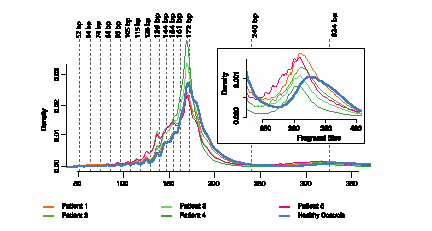
\includegraphics[width=0.9\linewidth]{Figures/intro/fragmentSizeDist}
\caption[Fragment size distribution of ctDNA]{Fragment size distribution of 5 high grade serous
ovarian carcinoma (HGSOC) patients and panel of healthy controls. The vertical dashed lines are placed on the fragment sizes between 52 and 172 bp where 10 bp periodicity is observed. The vertical lines at 240 and 324 bp show the range at which a shift in the di-nucleosomal peak occurs between HGSOC patients and healthy controls. The inset plot enlarges the density profile in the di-nucleosomal fragment length range. Figure adopted from \textcite{Markus2022}}\label{fig:ctdnaFragSize}
\end{figure}

Due to the different biological processes which can lead to the release of DNA from cancer cells, in addition to apoptosis, which is the \change{main}{primary} source of cfDNA from healthy cells, ctDNA has several biological differences from cfDNA. The most prominent features observed are distinct ctDNA fragmentation size patterns, fragment start sites, and fragment ends motives. While the preferred end motive and start site are heavily correlated, restricting the analysis to the lower tail of the mono- and di-nucleosomal peak of the fragment size distribution (74-155bp and 240-325bp) allowed a ctDNA tumour signal enrichment of at least 28\%. This \remove{is} enrichment and the high periodicity of the distribution showed a high dependence on nucleosomal placement. All ctDNA features combined were shown \remove{to be able} to predict the presence or absence of tumour DNA in samples regardless of tumour type  (\autoref{fig:ctdnaFragSize}, \cite{Mouliere2018,Markus2022}).

\add{Using the ctDNA contained in a blood sample as a non-invasive method of detection and monitoring of a patients cancer status has been used in many recent clinical trials, either to determine tissue of origin in cancers of unknown primary} \cite{Posner2022}\add{, predict clinical outcomes }\cite{Tan2019}\add{ and MRD detection. While ctDNA should theoretically be able to be used as a screening tool for early detection of cancers and risk groups, the general consensus is, that current methods are not sensitive enough for a population wide screening effort} \cite{CamposCarrillo2020,PonsBelda2021,Duffy2021}\add{.}
